\section{Control and Memory subsystem}
The control and memory subsystem of the accelerator can broadly be split into two parts - the frontend for fetching and executing the accelerator instructions and buffers for storing input and output maps. The frontend consists of task queues to which tasks are streamed into by the core, and configuration registers which store the runtime parameters of the current operation.

\subsection{Frontend}
The frontend consists of instruction queues, one queue for each type of instruction - LOAD, STORE, GEMM and ALU operation, with each instruction being 128-bit wide. The frontend has an instruction fetch module, which fetches instructions from the main memory by interacting with the interface module.

In addition, there is a load and a store unit that takes in the instruction from the command queue, contains address generation units that generates the relevant set of addresses to fetch from the main-memory and a dependency resolution module which resolves the dependency across instructions coming from the command queue. More on address generation and dependency resolution in section dealing with the instruction set. 


%To execute memory operations, the frontend module interacts with the interface module, which in turn interacts with the backend to load/store appropriate module. The GEMM/ALU instruction is dispatched to the systolic array / Tensor ALU respectively.

%The instructions in different queues have dependencies among them, which is set by the compiler when instructions are generated. The dependencies among the instructions have to be resolved manually by additional logic in the module. Once a dependency is resolved, it is dispatched to its corresponding module, as explained earlier.

\subsection{Buffers}
The buffers of relevance are Global buffer and Accumulator buffer, which store input maps and output maps respectively. Both buffers are banked structures, and hence support multiple accesses simultaneously.

%\begin{figure}[h]
%    \centering
%    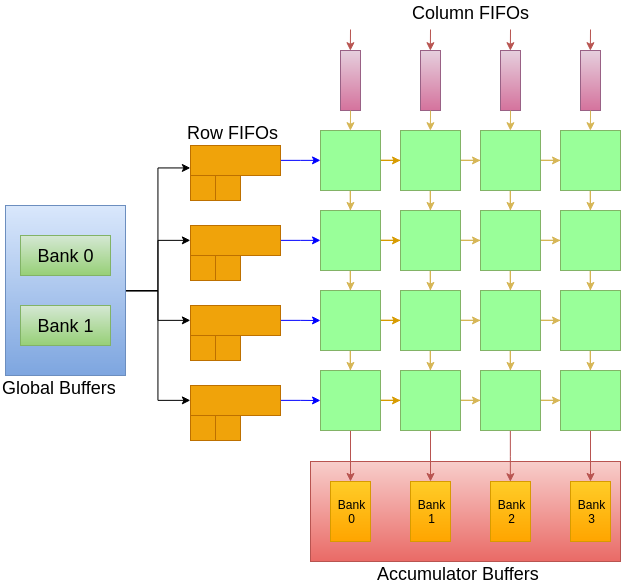
\includegraphics[scale=0.3]{images/peripheral.png}
%    \caption{Microarchitecture of systolic array with}
%    \label{fig:system}
%\end{figure}

\begin{enumerate}
    \item \textbf{Global buffer:} Global buffer is used to store input feature maps. The minimum number of banks in the global function is represented as $\frac{numRows}{filterRows}$, where numRows is the number of rows present in the systolic grid and filterRows is the number of rows of the filter matrix. To maximize utilization, in each cycle, one value should be sent into each row. Now, each input value will be used in filterRow number of convolution operations, and will contribute to value of filterRow number of output values. Hence, the above expression dictates the minimum number of banks in the global buffer, needed to maximize utilisation.
    
    \item \textbf{Accumulator buffer:} Accumulator buffer is used to store output feature maps. The minimum number of banks in the accumulator buffer is same as numCols, where numCols is the number of columns present in the systolic grid. Each column produces one output value per cycle, and hence, equal number of banks are needed to store them.
\end{enumerate}

\subsection{Design space}

\begin{enumerate}
    \item \textbf{Double buffering:} To hide memory latency of accessing input feature maps, double buffering can be used, in which the global buffer is duplicated. When input maps are read, it is first stored in buffer 0. Once sufficient data is read or buffer is full, the systolic read can start reading from buffer 0. In the meantime, the subsequent data needed can be simultaneously loaded into buffer 1. Once all values from buffer 0 are used, the buffers are switched (systolic grid starts reading from buffer 1, data is filled into buffer 0).
    
    \item \textbf{Double buffering weights in PE:} In the case of weight stationary dataflow explained earlier, the registers and datapaths of each PE, pertaining to weights, can be duplicated as well. By doing this, when one operation executes on the systolic array, the weights for the next operation can be loaded simultaneously and then control switched to read the new value loaded.
\end{enumerate}

